\documentclass[twocolumn]{article}
\usepackage[margin=1in]{geometry}

\usepackage{authblk}
\usepackage{pgfplots}
\usepackage{amsmath}
\usepackage{algorithm}
\usepackage{algpseudocode}
\usepackage{tikz}
\usepackage{pgfplots}
\usepackage{subcaption}
\usepackage{url}
\usepackage{cite}
\pgfplotsset{compat=1.18, width=7cm}

\title{Comparative Analysis Between Selection Sort and Merge Sort Algorithm}

\author{Nahid Niaz}
\author{Jobayer Mansur Mufti}
\author{Md. Shakibul Hasan}
\author{Md. Abdullah Al Mamun}
\author{Abir Chandra Das}
\author{Eazdan Mostafa Rafin}
\affil{Department of Computer Science and Engineering, Rajshahi University of Engineering and Technology}

\date{\today}

\begin{document}

\maketitle

\begin{abstract}
    In the realm of Computer Science, datasets are needed to sort according to different criteria.In order to solve these sorting problems, different sorting algorithms have been developed such as selection sort and merge sort.in this paper selection and merge sort algorithms were implemented on an octa-core processing machine using the $std::chrono()$ function and C++ language to compare their  respective execution time.The acquired results indicate that merge sort is more efficient and takes less execution time than selection sort, after testing several datasets of different sizes on the machine. For small input datasets, selection sort may be faster than merge sort. The central processing unit (CPU) plays a significant role in the performance of both algorithms.
    \\
    \textbf{Keywords:} Algorithms, Sorting, Merging, Complexity, Execution Time.

\end{abstract}


\section*{Introduction}
Sorting is the process of arranging data in a statistical order, which might be rising, decreasing, or lexicographical. In contrast, merging uses a divide-and-conquer strategy to sort a given array of components.

There are different types of sorting algorithms. Such as - insertion sort, bubble sort, selection sort, merge sort, quick sort, shell sort, tim sort, heap sort, and others. Each of them has a unique method for rearranging the elements, which improves the effectiveness and performance of the real-world applications while also making each one less time-consuming. A number of considerations need to be made when comparing different sorting algorithms. first of all, time complexity need to be considered as it establishes the maximum time that an algorithm can operate\cite{goodrich2010datap}. Many sorting algorithms, some of them are inefficient and excessively slow, depending on the size of data that needs to be rearranged. When expressing an algorithm's time complexity, big $O(n)$ notation is typically used, where O stands for complexity and n for the number of basic operations the algorithm performs\cite{jadoon2011design}. Then comes stability, which refers to the algorithm's capacity to maintain elements with equal values in the same relative order in the output as they did in the input\cite{ahmed2019stable}. Lastly, memory space is evaluated; recursive algorithms require more copies of sorting data, which affects memory space\cite{goodrich2010data}.

For situations involving small data sets, selection sort works especially well when there are few components and time complexity is not a major problem. When it comes to embedded systems—which have limited memory and processing power—its efficiency and simplicity make it a sensible option. In such contexts, the small code footprint and clear implementation of this technique are beneficial. Selection sort is also useful because of its simplicity as a tool for benchmarking and testing alternative sorting algorithms. For more complex sorting techniques in particular, it provides a baseline comparison. Furthermore, the method performs very well when used with partially sorted data since it saves needless swaps in segments that have already been sorted, which speeds up the sorting process. When changing components results in a substantial expense, the selection sort's efficiency is further enhanced in certain scenarios, including handling small keys and huge records, by its ability to reduce the number of swaps.\cite{scholarhat-selection-sort}

Merge sort is commonly used to efficiently sort big arrays of integers. Its versatility extends to external sorting, where it excels at managing enormous datasets that cannot fit into memory by separating and sorting smaller portions before merging them. Merge sort is useful in database operations for sorting data before searches, combining datasets, and optimizing queries. Its parallel processing capabilities allow it to be partitioned into sub-operations, enabling simultaneous execution and improving overall efficiency in computational tasks. Furthermore, merge sort is important in computer graphics, notably in-depth sorting, where it controls the order in which objects are drawn to build a 3D image, ultimately improving the quality of computer-generated visuals\cite{scholarhat-merge-sort}.


\section*{Background Study}
\subsection*{Selection sort}
Selection sort is a simple sorting algorithm.It works by repeatedly finding the minimum or maximum element in the unsorted part of the array and placing it in the sorted part.In each pass, one element will be sorted. For n elements, $n_1$ passes are required.
Firstly the algorithm sets the first element as minimum. Compare the minimum with the second element. If the second element is smaller than the minimum, assign the second element as the minimum. Compare minimum with the third element. Again, if the third element is smaller, then assign the minimum to the third element otherwise do nothing. Repeat this process until the last element. After each pass, minimum is placed in the front of the unsorted list. After each pass indexing starts from the first unsorted element. The algorithm can sort the array in ascending or descending order, depending on whether it finds the minimum or maximum element in each iteration\cite{programiz-selection-sort}.
This algorithm is not suitable for large data sets as its average and worst-case complexities are of $O(n^2)$, where n is the number of items and the space complexity is $O(1)$\cite{tutorialspoint-selection-sort}.

\begin{algorithm}
    \caption{Selection Sort}
    \begin{algorithmic}[1]
        \Procedure{SelectionSort}{$a, n$}
        \For{$i \gets 1$ to $n$}
        \State $j \gets i$
        \For{$k \gets i+1$ to $n$}
        \If{$a[k] < a[j]$}
        \State $j \gets k$
        \EndIf
        \EndFor
        \State $t \gets a[i]$
        \State $a[i] \gets a[j]$
        \State $a[j] \gets t$
        \EndFor
        \EndProcedure
    \end{algorithmic}
\end{algorithm}

\subsection*{Merge Sort}
Merge Sort is a divide-and-conquer algorithm that works by dividing the array into two halves, sorts each half independently, and then recombines them. The array is first split in half, and then each half is subjected to a recursive procedure until no more elements can be split. The sorting procedure starts after the array is split up into its smallest components. Every element is compared to its neighbor; if the elements do not match in order, they are exchanged. Finally, the sorted halves are combined once more, and the procedure is continued until the array is sorted in its whole. The average time complexity of merge sort is $O(n \log {n})$ where n is the number of items\cite{horowitz1998computer}. The auxiliary space complexity of this algorithm is $O(n)$\cite{geeksforgeeks-merge-sort}.

\begin{algorithm}
    \caption{Merge Sort}
    \begin{algorithmic}[1]
        \Procedure{MergeSort}{$low, high$}
        \If{$low < high$}
        \State $mid \gets \lfloor (low+high)/2 \rfloor$
        \State \textbf{MergeSort}($low, mid$)
        \State \textbf{MergeSort}($mid+1, high$)
        \State \textbf{Merge}($low, mid, high$)
        \EndIf
        \EndProcedure
    \end{algorithmic}
\end{algorithm}

\section*{Result and Analysis}
Running time of selection sort and merge sort algorithm using a different number of array sizes is
shown in Table \ref{selection-sort-graph} and \ref{merge-sort-table} respectively. And the graphical representation is shown in figure \ref{selection-sort-graph} and \ref{merge-sort-graph}.

\subsection*{Selection Sort}
\begin{table}[htp]
    \centering
    \caption{Running time of selection sort algorithm}
    \label{selection-sort-table}
    \begin{tabular}{|c|c|}
        \hline
        Array Size & Runtime (s) \\
        \hline
        10         & 0.0000008   \\
        \hline
        100        & 0.0000124   \\
        \hline
        1000       & 0.001009    \\
        \hline
        10000      & 0.0779707   \\
        \hline
        100000     & 9.02775     \\
        \hline
    \end{tabular}
\end{table}
\begin{figure}[htp]
    \centering
    \caption{Performance of selection sort algorithm}
    \label{selection-sort-graph}
    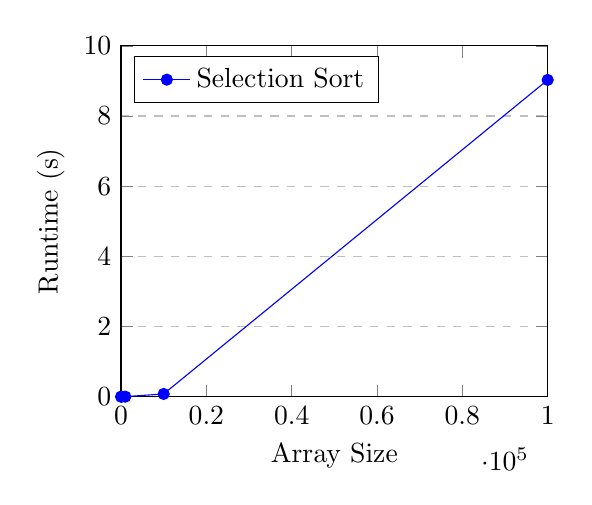
\begin{tikzpicture}
        \begin{axis}[
                xlabel={Array Size},
                ylabel={Runtime (s)},
                xmin=0, xmax=100000,
                ymin=0, ymax=10,
                xtick={0, 20000, 40000, 60000, 80000, 100000},
                ytick={0, 2, 4, 6, 8, 10},
                legend pos=north west,
                ymajorgrids=true,
                grid style=dashed,
            ]

            \addplot[
                color=blue,
                mark=*,
            ]
            coordinates {
                    (10, 0.0000008)
                    (100, 0.0000124)
                    (1000, 0.001009)
                    (10000, 0.0779707)
                    (100000, 9.02775)
                };
            \legend{Selection Sort}

        \end{axis}
    \end{tikzpicture}
\end{figure}

\newpage
\subsection*{Merge Sort}

\begin{table}[htp]
    \centering
    \caption{Running time of merge sort algorithm}
    \label{merge-sort-table}
    \begin{tabular}{|c|c|}
        \hline
        Array Size & Runtime (s) \\
        \hline
        10         & 0.000001    \\
        \hline
        100        & 0.0000055   \\
        \hline
        1000       & 0.0000055   \\
        \hline
        10000      & 0.0007045   \\
        \hline
        100000     & 0.0809197   \\
        \hline
    \end{tabular}
\end{table}
\begin{figure}[htp]
    \centering
    \caption{Performance of merge sort algorithm}
    \label{merge-sort-graph}
    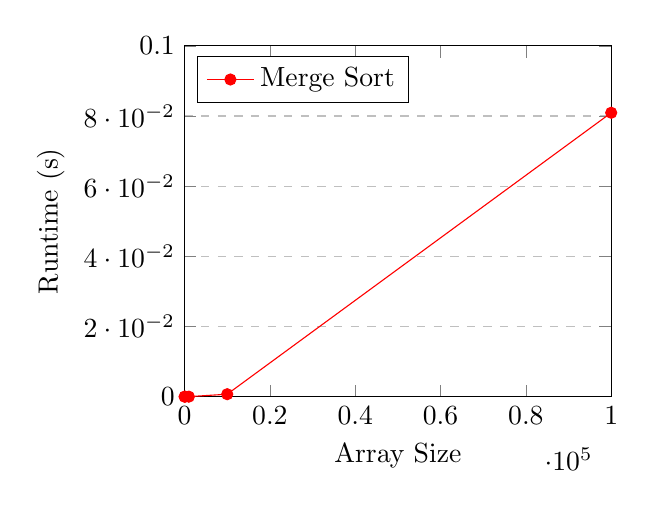
\begin{tikzpicture}
        \begin{axis}[
                xlabel={Array Size},
                ylabel={Runtime (s)},
                xmin=0, xmax=100000,
                ymin=0, ymax=0.1,
                xtick={0, 20000, 40000, 60000, 80000, 100000},
                ytick={0, 0.02, 0.04, 0.06, 0.08, 0.1},
                legend pos=north west,
                ymajorgrids=true,
                grid style=dashed,
            ]

            \addplot[
                color=red,
                mark=*,
            ]
            coordinates {
                    (10, 0.000001)
                    (100, 0.0000055)
                    (1000, 0.0000055)
                    (10000, 0.0007045)
                    (100000, 0.0809197)
                };
            \legend{Merge Sort}

        \end{axis}
    \end{tikzpicture}
\end{figure}

\begin{figure}[htp]
    \centering
    \caption{Performance comparison of selection sort and merge sort}
    \label{selection-merge-and-sort-graph}
    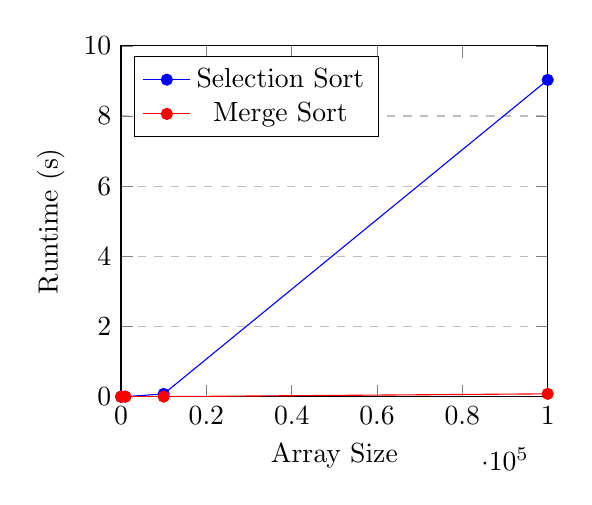
\begin{tikzpicture}
        \begin{axis}[
                xlabel={Array Size},
                ylabel={Runtime (s)},
                xmin=0, xmax=100000,
                ymin=0, ymax=10,
                xtick={0, 20000, 40000, 60000, 80000, 100000},
                ytick={0, 2, 4, 6, 8, 10},
                legend pos=north west,
                ymajorgrids=true,
                grid style=dashed,
            ]

            \addplot[
                color=blue,
                mark=*,
            ]
            coordinates {
                    (10, 0.0000008)
                    (100, 0.0000124)
                    (1000, 0.001009)
                    (10000, 0.0779707)
                    (100000, 9.02775)
                };
            \addlegendentry{Selection Sort}

            \addplot[
                color=red,
                mark=*,
            ]
            coordinates {
                    (10, 0.000001)
                    (100, 0.0000055)
                    (1000, 0.0000055)
                    (10000, 0.0007045)
                    (100000, 0.0809197)
                };
            \addlegendentry{Merge Sort}

        \end{axis}
    \end{tikzpicture}
\end{figure}

Selection Sort shows a steady rise in execution time with larger data sets.As its time complexity is $O(n^2)$.Merge Sort displays more steady and predictable behavior with a comparatively lower execution time rise as data set size grows, as it has better complexity than Selection Sort which is $O(n\log{n})$.
Table 1 and Figure 1 show that the running times of selection sort rise as the size of the array increases\cite{rabiu2018}. As a result, the durations required to sort a specific element in an array using selection sort are proportional to the number of elements in the array.
When the data size is 10000, the time required for selection sort is 0.0779707 seconds, but the time required for merge sort is 0.0007045 seconds, which is 110 times less than the time required for selection sort. When the data size was extended to 100000, the execution time for the selection sort increased to 9.02775 and the execution time for the merge sort increased to 0.0809197, which is 111 times smaller than the execution time for the selection sort.
Figure 3 shows that the Merge sort algorithm outperforms the Selection sort algorithm on both smaller and bigger array sizes throughout the sorting process.The performance of algorithms is affected by the array's input size\cite{rabiu2020}.

\newpage
\section*{Conclusion}
According to the study's findings, Merge Sort is more efficient and takes less time to execute than Selection Sort for large datasets. Selection Sort, on the other hand, may be faster than Merge Sort for small input datasets. The order of complexity of an algorithm affects its efficiency. The central processing unit (CPU) is critical to the performance of both methods. If the number of CPU cores is increased, the running time of both algorithms would decrease. As a result, these and other popular algorithms require further investigation to check if they provide the same results when tested on different machines.

\bibliographystyle{IEEEtran}
\bibliography{IEEEabrv,citation}

\end{document}
